% Options for packages loaded elsewhere
\PassOptionsToPackage{unicode}{hyperref}
\PassOptionsToPackage{hyphens}{url}
%
\documentclass[
]{book}
\usepackage{amsmath,amssymb}
\usepackage{lmodern}
\usepackage{ifxetex,ifluatex}
\ifnum 0\ifxetex 1\fi\ifluatex 1\fi=0 % if pdftex
  \usepackage[T1]{fontenc}
  \usepackage[utf8]{inputenc}
  \usepackage{textcomp} % provide euro and other symbols
\else % if luatex or xetex
  \usepackage{unicode-math}
  \defaultfontfeatures{Scale=MatchLowercase}
  \defaultfontfeatures[\rmfamily]{Ligatures=TeX,Scale=1}
\fi
% Use upquote if available, for straight quotes in verbatim environments
\IfFileExists{upquote.sty}{\usepackage{upquote}}{}
\IfFileExists{microtype.sty}{% use microtype if available
  \usepackage[]{microtype}
  \UseMicrotypeSet[protrusion]{basicmath} % disable protrusion for tt fonts
}{}
\makeatletter
\@ifundefined{KOMAClassName}{% if non-KOMA class
  \IfFileExists{parskip.sty}{%
    \usepackage{parskip}
  }{% else
    \setlength{\parindent}{0pt}
    \setlength{\parskip}{6pt plus 2pt minus 1pt}}
}{% if KOMA class
  \KOMAoptions{parskip=half}}
\makeatother
\usepackage{xcolor}
\IfFileExists{xurl.sty}{\usepackage{xurl}}{} % add URL line breaks if available
\IfFileExists{bookmark.sty}{\usepackage{bookmark}}{\usepackage{hyperref}}
\hypersetup{
  pdftitle={From Forests to Heritage: book of abstracts},
  pdfauthor={Kristof Haneca; Aoife Daly; Marta Domínguez-Delmás},
  hidelinks,
  pdfcreator={LaTeX via pandoc}}
\urlstyle{same} % disable monospaced font for URLs
\usepackage{longtable,booktabs,array}
\usepackage{calc} % for calculating minipage widths
% Correct order of tables after \paragraph or \subparagraph
\usepackage{etoolbox}
\makeatletter
\patchcmd\longtable{\par}{\if@noskipsec\mbox{}\fi\par}{}{}
\makeatother
% Allow footnotes in longtable head/foot
\IfFileExists{footnotehyper.sty}{\usepackage{footnotehyper}}{\usepackage{footnote}}
\makesavenoteenv{longtable}
\usepackage{graphicx}
\makeatletter
\def\maxwidth{\ifdim\Gin@nat@width>\linewidth\linewidth\else\Gin@nat@width\fi}
\def\maxheight{\ifdim\Gin@nat@height>\textheight\textheight\else\Gin@nat@height\fi}
\makeatother
% Scale images if necessary, so that they will not overflow the page
% margins by default, and it is still possible to overwrite the defaults
% using explicit options in \includegraphics[width, height, ...]{}
\setkeys{Gin}{width=\maxwidth,height=\maxheight,keepaspectratio}
% Set default figure placement to htbp
\makeatletter
\def\fps@figure{htbp}
\makeatother
\setlength{\emergencystretch}{3em} % prevent overfull lines
\providecommand{\tightlist}{%
  \setlength{\itemsep}{0pt}\setlength{\parskip}{0pt}}
\setcounter{secnumdepth}{5}
\usepackage{booktabs}
\ifluatex
  \usepackage{selnolig}  % disable illegal ligatures
\fi
\usepackage[]{natbib}
\bibliographystyle{plainnat}

\title{From Forests to Heritage: book of abstracts}
\author{Kristof Haneca \and Aoife Daly \and Marta Domínguez-Delmás}
\date{09 februari, 2022}

\begin{document}
\maketitle

{
\setcounter{tocdepth}{1}
\tableofcontents
}
\hypertarget{book-of-abstracts}{%
\chapter*{Book of abstracts}\label{book-of-abstracts}}
\addcontentsline{toc}{chapter}{Book of abstracts}

\begin{quote}
\textbf{From Forests to Heritage}

19-21 April 2022 - Amsterdam

\url{www.forests2heritage.nl}
\end{quote}

\href{./docs/forests2heritage.pdf}{download pdf}

\href{https://event.forests2heritage.nl/}{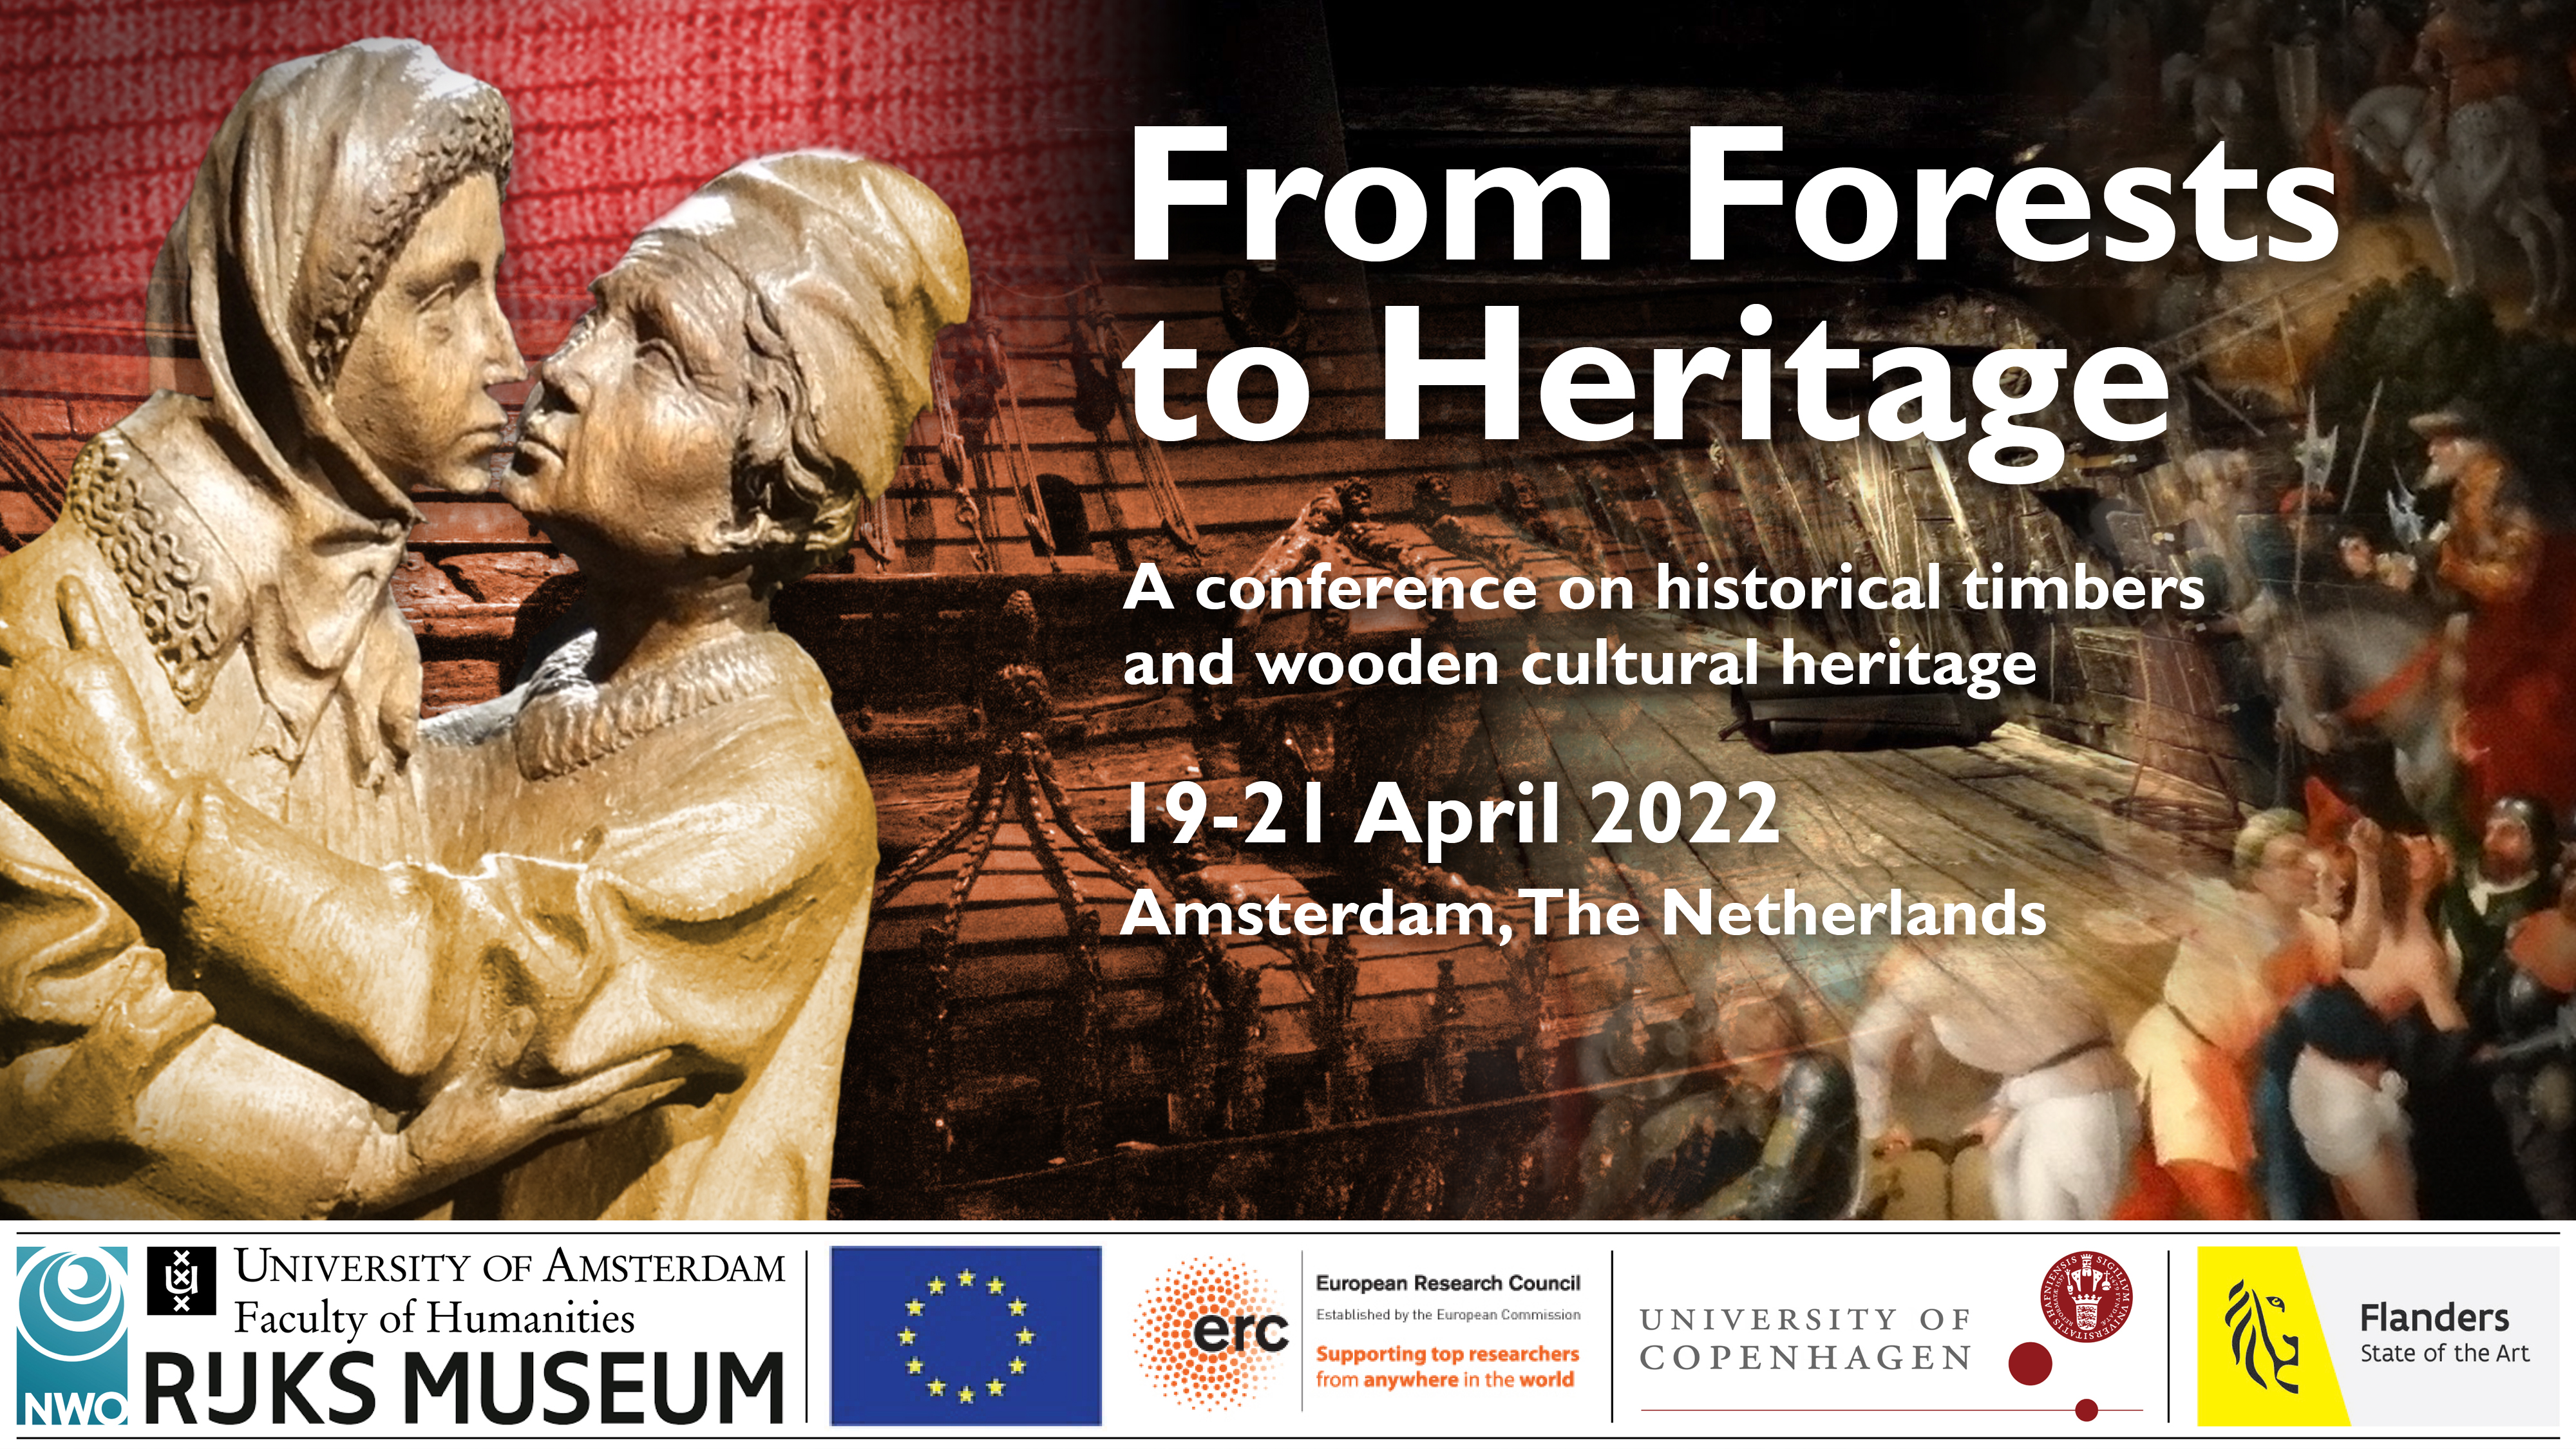
\includegraphics[width=1\textwidth,height=\textheight]{FORHER22_banner2.jpg}}

\hypertarget{part-program}{%
\part*{PROGRAM}\label{part-program}}
\addcontentsline{toc}{part}{PROGRAM}

\hypertarget{program}{%
\chapter*{Program}\label{program}}
\addcontentsline{toc}{chapter}{Program}

comming soon\ldots{}

\hypertarget{part-abstracts}{%
\part*{ABSTRACTS}\label{part-abstracts}}
\addcontentsline{toc}{part}{ABSTRACTS}

\hypertarget{session-1-forest-history}{%
\chapter*{Session 1: Forest history}\label{session-1-forest-history}}
\addcontentsline{toc}{chapter}{Session 1: Forest history}

\hypertarget{s1-o-001}{%
\section*{S1-O-001}\label{s1-o-001}}
\addcontentsline{toc}{section}{S1-O-001}

\textbf{Exploring the significance, acquisition and use of wooden resources
between Norse Greenland and North America: a (re)examination of literary
and archaeological sources}

Elie Pinta\textsuperscript{1}

\textsuperscript{1} Université Paris 1 Panthéon-Sorbonne, Paris, France -- UMR 8096.

\href{mailto:Elie.Pinta@etu.univ-paris1.fr}{\nolinkurl{Elie.Pinta@etu.univ-paris1.fr}}

Since prehistoric times, archaeological data reveal that wherever
forests are to be found, wood and timber are used to make furniture, to
construct buildings and ways of transportation, or as a fuel source.
While forestry practices, woodworking strategies or fuel gathering can
be studied through the archaeological records, historical documents are
also filled with information regarding the significance, acquisition,
and use of wooden resources. For example, much of the Scandinavian
peninsula was forested during the medieval period when Vikings, and the
later Norse, made the exploitation and transformation of wood and timber
one of their most distinguished crafts. Even during their migrations
across the tree-poor North Atlantic islands, Norse settlers kept relying
heavily on wooden materials for everyday use. Around AD 1000, as stated
in the so called Vínland Sagas, and supported by the findings at L'Anse
aux Meadows in northern Newfoundland, the Greenlandic Norse explored
part of the North American Atlantic coast, another heavily forested
area. Having been recognized as partly fictional, the Sagas - as well as
other literary descriptions -- can sometimes be treated with caution
regarding their historical accuracy. However, they also are filled with
ecological descriptions and technical information regarding the
exploitation of resources. Furthermore, archaeological data is sometimes
scarce or difficult to interpret due to methodological limitations.
Confronting both the textual and archaeological data provides a more
comprehensive understanding of wood culture in the Norse Greenlandic
world.

\hypertarget{s1-o-002}{%
\section*{S1-O-002}\label{s1-o-002}}
\addcontentsline{toc}{section}{S1-O-002}

\textbf{Reconstruction of economic resources associated with timber building
architecture in early medieval urban Trondheim}

Anna Helena Petersén\textsuperscript{1}

\textsuperscript{1} Norwegian Institute for Cultural Heritage (NIKU), Trondheim, Norway.

\href{mailto:anna.petersen@niku.no}{\nolinkurl{anna.petersen@niku.no}}

Timber buildings form a substantial part of the built environment in
medieval Scandinavia, both in rural and urban contexts. Because of often
favorable preservation conditions for organic material in urban
contexts, architectural remains are often encountered in the excavated
archaeological material from Norway's medieval towns. The past building
heritage can be reconstructed using archaeological sources,
cultural-historical information and expertise found in traditional
timber craftsmanship. Analyses of the volume of timber utilised in
buildings in urban contexts, and the types and development of
construction techniques used are important factors to be considered in
discussions of what an urban economy in medieval Norway consisted of.
However, timber as a natural resource is seldom included in studies of
urban medieval economy from an archaeological perspective. This
presentation uses the secular wooden architecture in early medieval
Trondheim (AD 950-1150) as a case to illustrate timber's role as an
economic resource, and highlights aspects of the socioeconomic
organisation the early urban Trondheim retrieved from remains of the
secular wooden architecture regarding access to timber, volumes of
timber used, and types of labour and skills employed.

\hypertarget{s1-o-003}{%
\section*{S1-O-003}\label{s1-o-003}}
\addcontentsline{toc}{section}{S1-O-003}

\textbf{A dendroecological reconstruction of forest management history in
Mediterranean \emph{Abies pinsapo} forests}

Linar Akhmetzyanov1, Raúl Sánchez-Salguero1, Pablo Casas-Gómez1, Víctor
Lechuga2, Benjamín Viñegla2, J. Julio Camarero3, José I. Seco1, José R.
Guzmán Álvarez4, José A. Carreira2, Juan C. Linares1

1 DendrOlavide, Depto. de Sistemas Físicos, Químicos y Naturales,
Universidad Pablo de Olavide, Sevilla, Spain. 2 Departamento de Biología
Animal, Vegetal y Ecología, Universidad de Jaén, Jaén, Spain. 3Instituto
Pirenaico De Ecología, Consejo Superior de Investigaciones Científicas
(IPE-CSIC), Zaragoza, Spain. 4 Dirección General del Medio Natural,
Biodiversidad y Espacios Protegidos. Consejería de Agricultura,
Ganadería y Desarrollo Sostenible. Junta de Andalucía, Sevilla, Spain.

\href{mailto:lakh@upo.es}{\nolinkurl{lakh@upo.es}}

Past disturbances related to forest-use history remain poorly understood
in long-term related Moroccan and Spanish fir forests. Here we
investigated tree recruitment, growth trends and abrupt changes in
tree-ring series of old-living trees since early 17th century in four
representative stands: Abies pinsapo in Grazalema and Sierra de las
Nieves (Spain) and A. marocana and A. tazaotana in Talassemtane
(Morocco). Retrospective dendrochronological analyses were supported by
documentary sources reporting changes in forest management and land-use
during the past 300 years. Age structures of each site were
discontinuous in time and revealed different cohorts distributed in
even-aged aggregated patches. Our results showed growth releases related
to past logging during the 18th, 19th and the early 20th century in
Spain and Morocco. Limited tree establishment from the 1940s to 1960s
agreed with intense herd grazing in Spain. Land-use changes leading to
grazing and logging limitations resulted in forest encroachment. The
observed patterns in growth releases allowed us to identify synchronous
past radial-growth releases due to forest management. Tree-ring series
have shown lower sensitivity to external disturbances, due to strong
drought susceptibility of Abies pinsapo, reflected in ``blue data''. Past
intensive selective cutting of the fir forest might also be reflected in
local historical buildings, opening new perspectives for
dendroarchaeological studies in the area.

\hypertarget{s1-o-004}{%
\section*{S1-O-004}\label{s1-o-004}}
\addcontentsline{toc}{section}{S1-O-004}

\textbf{Wood for funerary pyres in Barcino (Barcelona, NE Iberian Peninsula):
investigating cremation structures in two necropolis (1st-3rd centuries
CE) starting from charcoal analysis}

Sabrina Bianco1,2, Ethel Allué1,3, Santiago Riera Mora4, Emiliano
Hinojo5, Carme Miró Alaix6

1 Catalan Institute of Human Paleoecology and Social Evolution
(IPHES-CERCA), Tarragona, Spain. 2 Department of History and
Archaeology, Faculty of Geography and History, University of Barcelona,
Barcelona, Spain. 3 Department of History and Art History, University
Rovira and Virgili, Tarragona, Spain. 4 Seminaris d'Estudis i Recerques
Prehistòriques research group (SERP), Department of History and
Archaeology, Faculty of Geography and History, University of Barcelona,
Barcelona, Spain. 5 Freelance archaeologist, Barcelona, Spain. 6
Archaeological Service of Barcelona, responsible of Pla Bàrcino,
Direcció de Memòria, Història i Patrimoni -- Institut de Cultura (ICUB),
Barcelona, Spain.

\href{mailto:sbianco@iphes.cat}{\nolinkurl{sbianco@iphes.cat}}

Funerary rituals were an important part of the Roman cultural identity,
as they represent, with a precise set of rules and practices, the
passage from the world of livings to the deads. In this sense, fire
played a significant role, as a mean for cleansing the body and the soul
of the deceased through cremation, as well as for cooking funerary
banquets and offers. As consequence of the carbonization process, it is
possible to study the wood used for building the pyre and other goods
placed in the stake (rogus), as for example funerary beds (lecta
funebres), through wood charcoal analysis. In this work, the wood used
for cremations and funerary banquets in two suburban necropolis of the
colony of Barcino (Barcelona) will be discussed and compared. The first,
in use during the 1st century CE, was unearthed under St.~Antoni Market,
in relation with a main road (Via Augusta) that entered the roman city
from the west. It counted with several funerary enclosures where 2 busta
and 9 ustrina were identified. A second necropolis, functioning between
the 2nd-3rd centuries CE along another road, was excavated in Vila de
Madrid square, northwest from the city. In this case charcoal proceeding
from cremations (less abundant, as the practice decresed after the 2nd
century CE) or banquets, and two circular charred wooden structures have
been studied. Results of this investigation are significant because they
constitute the first sistematic study of wood use in roman funerary
contexts of Barcelona, up to now very limited to a few fragments.
Furthermore, this work evaluates wood selection practices based on
symbolic, functional or convenience criteria, the presence of wooden
objects/furnitures in the pyre and in general sheds light on the wood
management for supplying these rituals.

\hypertarget{s1-o-005}{%
\section*{S1-O-005}\label{s1-o-005}}
\addcontentsline{toc}{section}{S1-O-005}

\textbf{Woody resources and their management during Iron Age in northwest
Iberia}

María Martín-Seijo1

1 Departamento de Ciencias Históricas, Universidad de Cantabria,
Edificio Interfacultativo. Avda. de los Castros 52, 39005, Santander,
Spain.

\href{mailto:maria.martin@unican.es}{\nolinkurl{maria.martin@unican.es}}

Charcoal is the most common archaeobotanical remain recovered from
archaeological contexts dated to Iron Age in northern Iberia. This
presentation will summarise the results obtained from several
case-studies dated to the Iron Age in the northern part of the Iberian
Peninsula. Up to now, many charcoals have been analysed providing an
excellent opportunity to test the possibilities of going beyond
taxonomic identification. In our research we have systematically
combined charcoal analysis in tandem with registering dendrological and
taphonomic attributes. This has provided information to better
characterise the kind of woody resources managed, the combustion
process, the depositional and post-depositional processes affecting to
archaeobotanical assemblages. But it has also been obtained information
about wood uses, woodland management practices, and even about the
relationship established between people and their environment.

\hypertarget{s1-o-006}{%
\section*{S1-O-006}\label{s1-o-006}}
\addcontentsline{toc}{section}{S1-O-006}

\textbf{Sorting the trees: new evidences of woodland management at La Draga
(Banyoles, Spain)}

Oriol López-Bultó1, Patrick Gassmann2, Ingrid Bertin1, Raquel Piqué1

1 Department of Prehistory, Autonomous University of Barcelona,
Barcelona, Spain. 2 Independent researcher, Spain.

\href{mailto:oriollopezbulto@gmail.com}{\nolinkurl{oriollopezbulto@gmail.com}}

It is suggested that woodland management (e.g.~pollarding, pruning or
coppicing) was practised at least from the Neolithic onwards. The goal
of this presentation is to discuss woodland management practices in the
Early Neolithic waterlogged site of La Draga (5300-4700 cal BC -
Banyoles, Spain). So far different methods and techniques
(dendrochronology, roundwood age and diameter, dendrology\ldots) have been
applied to approach this issue and some preliminary results obtained.
But recent excavations brought forth new wooden archaeological materials
which help approach this issue from another point of view: the presence
of scars on the wood surface. For the first time, at la Draga, it has
been possible to identify scars on the wood surface of piles caused
after tool-marks and covered partially or totally by woundwood ribs,
indicating that the trees were marked before being cut down. The piles
marked have been identified as laurel (Laurus nobilis), this taxon is
well documented at the site (firewood, instruments and piles), although
playing a secondary role after oak. However, laurel is a tree rarely
exploited during the Neolithic in Europe, which poses the question of
the intentional selection of this wood at La Draga. This paper will
present the results of the morphological, technological and
dendrological study of the laurel piles in the context of the wooden
remains of La Draga site. The results of the different approaches are
summarized and contrasted to provide new lights on Neolithic woodland
management in Europe. Moreover, it is discussed the role of the laurel
tree in the context of the Neolithic.

\hypertarget{s1-o-007}{%
\section*{S1-O-007}\label{s1-o-007}}
\addcontentsline{toc}{section}{S1-O-007}

\textbf{From the exhaustive study of a mountain village to the restitution of
forest: how far can dendrochronology go?}

Lisa Shindo1

1 ROOTS Cluster of Excellence, Institute of Pre- and Early Prehistoric
Archaeology, Christian-Albrechts-University, Kiel, Germany.

\href{mailto:lshindo@roots.uni-kiel.de}{\nolinkurl{lshindo@roots.uni-kiel.de}}

Since 2014, as part of several research projects on the links between
humans and forests in the past, 20 buildings in a village in the
southern French Alps (Courbons, 900 m altitude) have been studied by
dendrochronology. These are mainly village houses but also a church, a
bell tower and a mill. We were interested in the wood used in the
structural work, which is only present in the ceilings. These are mostly
joisted, but two of them are more elaborated, with visible beams and
joists. A total of 155 timbers were studied. The species used are very
varied, oak, fir, larch, Scots pine, elm, ash and willow or poplar, as
are the growth patterns and felling dates, which range from the 14th to
the 19th century. Although the village is mentioned in texts as early as
the 12th century, the main felling phases take place in the 15th and
18th centuries (the study of these timbers contributed to the
construction of the first oak reference curve at altitude in the
southern French Alps). According to the texts, since at least the 15th
century, local wood has been exported to the lowland cities and is at
the heart of a very active local market. As we have observed a change in
the wood used in the 16th c., we will address the issues of wood
resources and forestry management in this region at the crossroads of
several trade routes, linking the high mountains, the plains and the
Mediterranean Sea.

\hypertarget{s1-p-001}{%
\section*{S1-P-001}\label{s1-p-001}}
\addcontentsline{toc}{section}{S1-P-001}

\textbf{Our history does not exist in the books: forest patches framing new
identities for heritage and environmental conservation}

Pascoal Gota1, Anneli Ekblom1

1Department of Archaeology and Ancient History, Faculty of Arts, Uppsala
University/ Uppsala, Sweden.

\href{mailto:pascoal.gota@arkeologi.uu.se}{\nolinkurl{pascoal.gota@arkeologi.uu.se}}

With the huge increase of illegal logging activities globally, forests
that are not in the borders of officially designated conservation areas
are currently at risk of being classified, simplified and reduced to
spaces for logging. In the best case scenario, these forests can be
spared either through conservation protection (which tends to exclude
local communities) or through a re-categorisation as sources for
ecosystem services of benefit for several stakeholders. Forest patches
play a fundamental role in ensuring the existence of several ecosystem
services. In this paper we bring into discussion the results of field
work carried in two of the several forest patches located in southern
Mozambique. Methodologically, we approach forest patches as cultural
landscapes and heritage sites. Our aim is to formulate an approach of
biodiversity conservation that goes beyond officially protected areas,
such as parks and reserves in collaboration with local communities
through the notion of protected cultural landscapes and bicultural
heritage. In doing so, we documented the histories of these forest
patches as embedded in social memories and physical remains (pollen,
charcoal and archaeological finds) to narrate the role of forest mosaics
in shaping the identity of current communities. With our findings, we
illustrate that the local conservation of these forests is effective,
resting on tangible and intangible protection of heritage a practice
fundamental for the identity of custodian communities. We conclude by
providing some insights for the study and understanding of
transdisciplinarity and conservation as these protected forests are
potential bridges to dialogue and community-based heritage-conservation
initiatives through collaborative approaches to achieve several of the
sustainable development goals.

\hypertarget{s1-p-002}{%
\section*{S1-P-002}\label{s1-p-002}}
\addcontentsline{toc}{section}{S1-P-002}

\textbf{Mechanical wood properties over the past 100 years}

Andreas Rais1, Andriy Kovryga1, Jan-Willem G. van de Kuilen1,2

1 Materials Engineering, School of Engineering and Design, TU Munich,
Munich, Germany. 2 Engineering Structures, Biobased Structures and
Materials, TU Delft, Delft, the Netherlands.

\href{mailto:rais@tum.de}{\nolinkurl{rais@tum.de}}

Forest stands adapt their growth on changes of temperature, nitrogen
deposition, CO2-concentration and growing season. Forest management
strategies also influence tree growth, for instance by admixing
deciduous trees in coniferous forests or reducing rotation age and stand
density. Climate change by itself or indirectly through silvicultural
adaptations may have influenced the wood (mechanical) properties. The
focus of this study is on Norway spruce (Picea abies), which is relevant
for use in construction despite the climate and calamity-related decline
in European forests. Our internal database contains data about strength,
stiffness, density and knot parameters from more than 10.000 boards.
Most of the data were collected in order to derive models and threshold
values for structural engineering applications, and as such can be
considered representative of the timber grown in Central Europe in the
last two centuries. From each of these boards, a small, defect-free wood
sample is available to determine the date of wood formation
(dendrochronological approach) and essential growth ring
characteristics. The presentation highlights the methods, but also gives
first insights into whether mechanical wood properties may have changed
in the last century. Changes in wood quality due to climate and
management concepts are important for the entire wood processing chain
forest-sawmill-final product. As the log and wood quality determine the
product performance, any changes have a direct impact on the production
chain and the added value during each production step. Sawmills notice a
change in timber quality due to changed yields in the various
assortments that they produce affecting revenue.

\hypertarget{s1-p-003}{%
\section*{S1-P-003}\label{s1-p-003}}
\addcontentsline{toc}{section}{S1-P-003}

\textbf{Dendrochronological investigation of monumental trees from ``Villa
Medicea di Castello'' in Florence, Italy}

Sveva Longo1, Cristiano Riminesi1, Rachele Manganelli del Fà1, Silvia
Fineschi1, Giovanna Battipaglia2 1 Institute of Heritage Science,
National Research Council of Italy, Italy. 2 Department of
Environmental, Biological, Pharmaceutical Sciences and Technologies,
University of Campania ``Luigi Vanvitelli'', Caserta, Italy.

\href{mailto:sveva.longo@ispc.cnr.it}{\nolinkurl{sveva.longo@ispc.cnr.it}}

The garden of the Villa Medicea of Castello was designed by Niccolò
Tribolo in 1538 on commission of Cosimo I de' Medici, Gran Duke of
Florence, and represents one of the prototypes of the XVI century
Italian garden. A cycle of `lunettes' painted by the Flemish artist
Iustus van Utens between 1599 and 1603 illustrate fourteen villas
belonging to the Medici Family, including this one. In this study, we
performed dendrochronological analysis on two pubescent oaks, Quercus
pubescens Willd, from the ``Piano del selvatico'', to verify whether they
might be dated back to the garden origin. This analysis would provide
important information on the vegetation history of the garden, and fill
lack of records about its past management. Two trees, ranging in size
from 100 to 150 cm diameter at breast height, were sampled. Two cores
for each plant were collected in summer 2021 using an increment borer
(Haglöfs, Sweden) of 5 mm. Results revealed that both trees show evident
signs of senescence, with rotting of the wood in the central part and
have undergone several pest attacks during their existence. It was not
possible to reach the center of the trunk due to the presence of rotten
wood, therefore the missing rings were estimated by allometric equation
to define the age of the two oaks. The age was determined about 500
years old. The estimated age of two pubescent oaks allows us to affirm
that they were already present when the `lunettes' were painted.

\hypertarget{s1-p-004}{%
\section*{S1-P-004}\label{s1-p-004}}
\addcontentsline{toc}{section}{S1-P-004}

\textbf{History of wood management}

Caroline Vermeeren1, Kirsti Hänninen, Welmoed A. Out2 1 BIAX Consult,
Research centre, Zaandam, the Netherlands. 2 Moesgaard Museum, Aarhus,
Denmark.

\href{mailto:vermeeren@biax.nl}{\nolinkurl{vermeeren@biax.nl}}

From written and iconographic sources there is proof for wood management
in the historical period, but when did this practice start? It is often
assumed that this could have been as far back as the Neolithic. To
investigate this, a model was made using the combination of diameter and
number of annual rings (figure 1). Management (pollarding and coppicing)
results in a higher quantity and quality of wood, due to better access
to light. Managed trees are supposed to grow faster, producing thicker
annual rings. This was tested on modern trees resulting in reference
graphs per taxon. Case studies for the Neolithic from different parts of
Europe, are compared to these graphs of which some will be presented. A
management signal could not be found. Different possibilities are
discussed to explain this result.

\hypertarget{session-2-shipwrecks-and-archaeological-structures}{%
\chapter*{Session 2: Shipwrecks and archaeological structures}\label{session-2-shipwrecks-and-archaeological-structures}}
\addcontentsline{toc}{chapter}{Session 2: Shipwrecks and archaeological structures}

\hypertarget{s2-o-001}{%
\section*{S2-O-001}\label{s2-o-001}}
\addcontentsline{toc}{section}{S2-O-001}

\textbf{Piers, wharfs and shipping at Masthugget, Gothenburg -- Investigating private harbours through wood and stone structures}

Andrine Nilsen1

1 Rio Göteborg Natur- \& kulturkooperativ, Gothenburg, Sweden.

\href{mailto:andrine.nilsen@riogbg.se}{\nolinkurl{andrine.nilsen@riogbg.se}}

The harbour area Masthugget have large timber collections and stone structures as its main archaeological features. This contract archaeological project investigates how the built environment changes in character in different parts of the harbour from enterprise oriented to large private estates with lush gardens. The dendrochronological analysis is of vital importance to the project linked to dating, wood provenance analysis, the inquiry into timber supplies as well as for the study of the reconstruction and development of the harbour. Dendrochronology also plays part in the dating of the building stock on the piers and plots. Other dating tools used to track the 17-19th century are archaeological finds analysis combined with historical maps of the area. Most plots and piers were private, and the owners were to a high degree well-known tradesmen many with Scottish origin. The city also owned two of the piers, one used as an iron-weighing station. In many ways, the harbours expands and benefits from international trading blockades connected to wars between England, France and North America affecting the colonial trade. The harbour was used for the import of colonial goods while exports such as tea, herring, iron and whale-oil were the most important. Other significant exports were timber and masts (which gave the harbour its name). The project aims to find out how this foremost private harbour changed over time, how it was used, what the building stock of the piers looked like and how the buildings connected to the various enterprises of the area.

\hypertarget{s2-o-002}{%
\section*{S2-O-002}\label{s2-o-002}}
\addcontentsline{toc}{section}{S2-O-002}

\textbf{Marking time in the Iron Age; the dendrochronology of loch (lake) settlement in SW Scotland}

Anne Crone1

1 AOC Archaeology Group, Unit 7A Edgefield Industrial Estate, Loanhead, Midlothian, Scotland.

\href{mailto:anne.crone@aocarchaeology.com}{\nolinkurl{anne.crone@aocarchaeology.com}}

Although there is evidence for settlements in the lochs of Scotland from the Neolithic to the early modern period, the 1st millennium BC saw the most intense period of activity, specifically that period from 800 to 400 BC where the calibration curve is so flat as to render radiocarbon determinations highly imprecise. Studies of the Iron Age throughout Europe are bedevilled by the Halstatt Plateau but in the British Isles few sites of that period have benefitted from the precision of dendro-dating. However, in a small area of SW Scotland, there are now three dendro-dated wetland settlements which are enabling archaeologists to examine the dynamics of regional settlement development via the chronological relationships between these sites. Extensive excavations at one of these sites, Black Loch of Myrton, yielded large quantities of oak, alder, hazel and ash, all of which have been analysed to produce a precisely dated chronological framework spanning three major episodes of occupation on the settlement, from 438/7 BC to 223 BC. Over the course of two centuries we see the development, expansion, abandonment and re-occupation of the settlement, all at the scale of human lifetimes. In this talk the dendrochronological evidence from SW Scotland will be outlined, and some of the interpretative issues associated with the use of non-oak species will be raised. The impact of high-resolution timescales on our understanding of the dynamics of settlement in this period will also be explored.

\hypertarget{s2-o-003}{%
\section*{S2-O-003}\label{s2-o-003}}
\addcontentsline{toc}{section}{S2-O-003}

\textbf{Just bad quality? Some thoughts on the use of timber in medieval to modern shipbuilding}

Mike Belasus1

1 Lower Saxony Institute for Historical Coastal Research, Wilhelmshaven, Germany.

\href{mailto:belasus@nihk.de}{\nolinkurl{belasus@nihk.de}}

The perception of wood in connection to shipbuilding of the past seems to be strongly idealised and often not fitting to the reality reflected in the archaeological context. Features of tree-anatomy were only sometimes recorded, and often ignored during the interpretation of ship finds. The idealized idea of a shipwright, who is choosing personally only the best material, was likely born out of an idealized image of the past and possibly influenced by rather recent shipbuilding practices. Detailed advise on the choice of high quality timbers for shipbuilding only appear in the 20th century, long after wood was superseded by steel for most vessels and competition for shipbuilding timber on the marked market had ceased. In some cases, this has produced a somewhat distorted interpretation of ships and shipbuilding because features of growth, in a holistic approach, can give information beyond timber quality but also on environmental influences and the human impact on this resource. In certain cases, it even allows to draw conclusions on economic and social circumstances. This way the information gathered from the building timber can alter the vessels interpretation. This paper will discuss the demands for shipbuilding timber and its quality in North Western Europe as a result of the ERC-TIMBER project (Grant agreement No.~677152). It aims to reflect on possible social, economic or environmental reasons for the shipwrights' choices.

\hypertarget{s2-o-004}{%
\section*{S2-O-004}\label{s2-o-004}}
\addcontentsline{toc}{section}{S2-O-004}

\textbf{Double checking double Dutch: A reassessment of the construction features of the early modern Scheurrak SO1 shipwreck}

Rik Lettany1 , Petra Doeve2, Esther Jansma3

1 Department of World Archaeology, Faculty of Archaeology, Leiden University, Leiden, the Netherlands. 2 BAAC Archeologie en Bouwhistorie. 3 Cultural Heritage Agency of the Netherlands.

\href{mailto:h.lettany@arch.leidenuniv.nl}{\nolinkurl{h.lettany@arch.leidenuniv.nl}}

In 1984, the remains of a late 16th Century Dutch merchantman were discovered off the coast of Texel, the Netherlands. The excavation of the site, named Scheurrak SO1 after its location, started in 1988 and ended in 1997. With a strong focus on the ship's construction features, it became one of the pioneering projects of Dutch underwater archaeology. The shipwreck exhibited several peculiar construction details which deviated from other contemporary European shipbuilding traditions. As such, the data recovered from the Scheurrak SO1 shipwreck contributed strongly to what in nautical archaeology became known as the Dutch Flush and the Double Dutch discourses. Dutch flush refers to the shell-first building sequence of Dutch carvel built ships, at a time that most shipbuilding traditions used a frame-first sequence. Double Dutch, then again, refers to a brief moment in time when Dutch flush ships were built with a double layer of planking. Scheurrak SO1 has been considered the earliest known example of this latter technique. Based upon very limited dendrochronological data, the initial hypothesis was that Scheurrak SO1 was built around 1580 with two layers of planking. Reassessment of Scheurrak SO1's construction details within the frame of the interdisciplinary research project ``Scheurrak SO1 in the Maritime Cultural Landscape of the Early Modern Netherlands, 1550-1650'' at Leiden University, now suggests that the ship may have known multiple building phases. Re-analysis of the available tree-ring curves seems to support this, while analysis of additional samples demonstrate a more dispersed timber provenance than initially deduced. Although research is still ongoing, current results do challenge the known Double Dutch discourse and encourage a reinterpretation of the construction of the Scheurrak SO1 shipwreck.

\hypertarget{s2-o-005}{%
\section*{S2-O-005}\label{s2-o-005}}
\addcontentsline{toc}{section}{S2-O-005}

\textbf{From a forest to a ship and into a wreck, and back again?}

Minna Koivikko1, Tuomas Aakala2, Katariina Vuori3

1 Finnish Heritage Agency, Finland. 2 Department, Jyväskylä, Finland. 3 Department, Oulu, Finland.

\href{mailto:minna.koivikko@museovirasto.fi}{\nolinkurl{minna.koivikko@museovirasto.fi}}

The aim of the project is to develop interpretation of so-called skeleton wrecks, i.e., wooden wrecks, which only have preserved partly, and no informative objects have been discovered. We are studing the relationship between a man and a forest through interpretation of wooden vessels. The Lost Navy, Sweden's ``Blue'' Heritage c.~1450--1850 research programme aims to collect information about the ships in the fleet. It is a joint marine archaeology and - history project in the Baltic Sea region for 2021--2026. In Finland, the research sub-project focuses on wooden wrecks of the Swedish era fleet. The project has a multidisciplinary approach, combining archaeology with shipbuilding, dendrochronology, and forest studies.

\hypertarget{s2-o-006}{%
\section*{S2-O-006}\label{s2-o-006}}
\addcontentsline{toc}{section}{S2-O-006}

\textbf{Wood identification and dendrochronological techniques applied for the study of shipwrecks on the Atlantic coast of Argentina: comparison of different case studies showing limitations and potentials}

Ignacio A. Mundo1,2

1 Laboratorio de Dendrocronología e Historia Ambiental, IANIGLA/CONICET, Mendoza, Argentina. 2 Facultad de Ciencias Exactas y Naturales, Universidad Nacional de Cuyo, Mendoza, Argentina.

\href{mailto:iamundo@mendoza-conicet.gob.ar}{\nolinkurl{iamundo@mendoza-conicet.gob.ar}}

Wood anatomy or xylogeny allows the botanical identification of woody material based on the recognition and quantification of various wooden traits. In the case of archaeology, and in particular for nautical archaeology, the wood anatomy provides information on the possible origin of nautical structures based on the range of distribution of woody plants, allows the association between the function fulfilled by a piece within a vessel and the mechanical properties of the wood, and it also helps to evaluate aspects related to the availability of timber and the building technology of a shipwreck, among others. In a nautical archaeological sense, dendrochronology analyses the information recorded in tree rings of timbers, which allows the dating of woody materials used in ship building, as well as estimating their possible origin (i.e.~dendroprovenancing). In this context, the interdisciplinary work between these three disciplines (xylogeny, dendrochronology and nautical archaeology) has only recently been applied in Argentina, despite the existence of a large number of woody nautical remains on the extensive Atlantic coast of this country. Through the analysis of different case studies carried out in the last years, this presentation aims to present and discuss the scope and limitations of the wood anatomy analyses in underwater archaeological studies in Argentina as well as to emphasize the dendroarchaeological potential of some of the materials found. The characteristics of the materials analysed in each case will be summarised, highlighting the limitations encountered and the potentialities for future studies.

\hypertarget{s2-o-007}{%
\section*{S2-O-007}\label{s2-o-007}}
\addcontentsline{toc}{section}{S2-O-007}

\textbf{House and Boat. Reuse of ship planking in a 10th century building at Hungate, York}

Steven J. Allen1

1 Conservation Department, York Archaeology.

\href{mailto:sallen@yorkat.co.uk}{\nolinkurl{sallen@yorkat.co.uk}}

In the course of excavations by York Archaeological Trust (Now York Archaeology) in 2008-9 at Hungate in York revealed the waterlogged timbers of another building of a type best known from Coppergate. This building, dating to the third quarter of the 10th century CE was superficially of the same construction as seen earlier at Coppergate and was a rectangular pit cut into the ground, lined with posts that supported a boarded outer lining. At Coppergate, the timbers were largely freshly felled specifically for the buildings in which they were found and the tree ring sequences are local to the York region. However at Hungate, when the timbers were lifted, it was immediately apparent that the board lining was in fact made up of reused articulated slabs from a clinker-built boat. Moreover, the type of clinker construction was unusual and not of the `typical' North West European/Scandinavian type. Dendrochronological samples allowed the identification of the potential source for the boat timbers, which was not local to York. This paper considers the evidence provided from the study of the woodworking technology and the work done to identify the type of boat, its potential provenance and indeed the provenance of the timbers used in its construction.

\hypertarget{s2-o-008}{%
\section*{S2-O-008}\label{s2-o-008}}
\addcontentsline{toc}{section}{S2-O-008}

\textbf{How a broken wooden board uncovered an early medieval mill}

Julia Weidemüller1, Franz Herzig1, Leander Schmidt1, Jeremy Collacott1

1 Bayerisches Landesamt für Denkmalpflege, Thierhaupten, Germany.

\href{mailto:julia.weidemueller@blfd.bayern.de}{\nolinkurl{julia.weidemueller@blfd.bayern.de}}

In September 2021, historic timbers were uncovered at a construction site in Aichach, Bavaria. The site was not designated as monument, therefore it was not accompanied archaeologically. Nevertheless, the construction company reported these finds to the Bavarian State Office for Monument Preservation (BLfD). The first pieces were examined in the internal laboratory for dendroarchaeology. The site could be identified as an early medieval mill on the basis of a broken paddle fragment. Subsequently, hundreds of timbers from several construction phases of the mill were excavated and documented in close cooperation between Construction Company, Archaeological Specialists and Dendroarchaeologists. In addition to small finds such as paddles, vessels and tools, numerous construction timbers were found, many still in situ. For the first time, an intact mill pond, including dam, filter system and mill channel, could be excavated. In this case the wood species composition is exciting, since a large part of the construction timbers consisted of alder and beech. Only heavily used structures like the sluice gate or the substructures of the mill building were made of oak. The investigations have not yet been completed. First measurements date to the 8th and 9th centuries AD. A heavy flood event ended milling at this site. A comprehensive archaeological evaluation is planned, including age structures and wood species composition. However, the sheer mass of the timbers would offer many more starting points for statistical analyses on early medieval forest structures and wood species selection, to name a few. Since there are no resources available at BLfD for research of this kind, I hope that the presentation of the project to expert circles will provide helpful comments and possibly lead to further research.

\hypertarget{s2-o-009}{%
\section*{S2-O-009}\label{s2-o-009}}
\addcontentsline{toc}{section}{S2-O-009}

\textbf{A dendroarchaeological study of Roman-period river barges from the Lower Rhine region}

Yardeni Vorst1

1 Vorst wood research, Zaandam, the Netherlands.

\href{mailto:yvorst@gmail.com}{\nolinkurl{yvorst@gmail.com}}

In 2003, a river barge dating to the Roman period was found in a former riverbed of the Rhine in the western part of the Netherlands. The ship, named `Woerden 7', formed a new discovery in a long series of Roman-period ship finds in Lower Rhine region since the late 1960's. In particular, large flat-bottomed river barges had been found. Many of these vessels were excavated and some were conserved, such as the The Zwammerdam ships, found in the village of Zwammerdam in the 1970's. For a research project these ships have been re-examined using more modern techniques. A comparison between ship Zwammerdam 6 and the earlier mentioned Woerden 7 vessel shows that the ships resemble each other closely in construction. Apart from a study of the ship constructions a dendroarchaeological study of the timbers has been undertaken. Dendrochronology has been used to date the ships and to determine which timbers were obtained from the same trees. This has helped to trace original building sequences and allowed for new ideas on the shipbuilding processes. Identifying the source area of trees used in this Roman-period shipbuilding, i.e.~the provenance of the timbers will be presented in an other paper together with Ronald Visser. The Zwammerdam vessels are currently being reconstructed at an archaeological park (Archeon) in the South of Holland and the research information gathered will contribute to stories on their historical background.

\hypertarget{s2-p-001}{%
\section*{S2-P-001}\label{s2-p-001}}
\addcontentsline{toc}{section}{S2-P-001}

\textbf{Conservation processes of a painted wooden coffin at Saqqara area}

Abdelmoniem M. Abdelmoniem1 , Naglaa Mahmoud1, Wael S. Mohamed2,

1Conservation Department, Faculty of Archaeology, Fayoum University, Fayoum, Egypt. 2 Polymer department, National Research Centre, Dokki, Giza, Egypt.

\href{mailto:ama63@fayoum.edu.eg}{\nolinkurl{ama63@fayoum.edu.eg}}

This paper aims to document the conservation processes of a polychrome wooden coffin at Saqqara dating back to the late period. The exterior part of the coffin is decorated with painted layer, while inside it is covered with a layer of the black resin. The coffin was in a bad condition. It was covered with a thick layer of dust, loosing parts of the painted and gesso layers, as well as other parts of these layers were lost. Some parts were missing from the foot area of the lid coffin. 2D illustrations and 3D modules were made to document the coffin. The conservation processes of the wooden coffin included mechanical and chemical cleaning, reattachment of the separated parts of the ground layer and painted layers, filling the edge of the painted layer, and consolidating the black resin layer. The materials used for these processes proved to be stable and retrieval by many researchers. The conservation process included mechanical cleaning using soft brushes, chemical cleaning using ethyl alcohol and water for painted layer and xylene and water for black resin layer, stabilization of the separated gesso layer using Paraloid B72, filling cracks of the gesso layers using glass microballoon with Paraloid B72, and consolidating the painted layer with KlucelE and black resin layer with Nano Paraloid B72.

\hypertarget{s2-p-002}{%
\section*{S2-P-002}\label{s2-p-002}}
\addcontentsline{toc}{section}{S2-P-002}

\textbf{Microscopy techniques for the examination of waterlogged archaeological wood}

Angela Balzano1, Maks Merela1, Katarina Čufar1

1 Biotechnical Faculty, University of Ljubljana, SI1000 Ljubljana, Slovenia.

\href{mailto:Angela.Balzano@bf.uni-lj.si}{\nolinkurl{Angela.Balzano@bf.uni-lj.si}}

Waterlogged archaeological wood (WAW) from prehistoric pile-dwelling settlements in Ljubljansko barje, Slovenia, was examined using various microscopic techniques. We have performed light microscopy (LM) using bright field, polarization and fluorescence modes with different sample preparation methods (cutting of frozen WAW, cutting after embedding in paraffin). Unstained and stained sections with safranin and astra blue or acridine orange and chrysoidin were considered. We have developed an improved protocol for scanning electron microscopy (SEM) and energy dispersive X-ray spectroscopy (EDX) based on the observation of sections obtained with a razor blade from frozen samples and fixed with albumin on sample supports to prevent cracking and collapse of the highly degraded wood. Advantages of applied techniques will be shown for WAW of Quercus, Faxinus, Acer, Salix and Populus with an age of about 4,500 years. Sections from frozen WAW, approximately 20-30 µm thick and 1cm2 in size, allowed recognition of cellular and tissue level structures with LM. Embedding in paraffin provided thinner but smaller sections which tended to tear. The improved SEM protocol provided high quality images of large sections at lower magnifications and also of details at high magnifications with high resolution. The combination of SEM and EDX allowed the observation of the preservation of the cell wall as well as the location, amount, shape and chemical composition of various inclusions with high amounts of Fe, S and Ca found in all taxa studied, while Populus also contained increased amounts of Si.

\hypertarget{s2-p-003}{%
\section*{S2-P-003}\label{s2-p-003}}
\addcontentsline{toc}{section}{S2-P-003}

\textbf{Practices of shipwreck timber sampling for dendrochronology}

Daniel Peter Dalicsek1

1 Moesgård Museum, Aarhus, Denmark.

\href{mailto:dad@moesgaardmuseum.dk}{\nolinkurl{dad@moesgaardmuseum.dk}}

In 2018, two important publications saw light, Selecting and Sampling Shipwreck Timbers for Dendrochronological Research: practical guidance by Daly et al.~and Shipwrecks and Provenance: in-situ timber sampling protocols, with a focus on wrecks of the Iberian shipbuilding tradition by Rich et al.~My presentation would look at the impact of these publications and the focus on the works of maritime archaeologists and dendrochronologists in sampling shipwreck timbers over the past five years. It´s main focus would be on intrusive survey methods and on shipwreck sites, but would not exclude other underwater sites or terrestrial excavations. It would consist of a survey questionnaire, sent out to maritime archaeologists across the globe and interviews with maritime archaeologists and dendrochronologists ahead of the conference. This would enable insight and provide an overview over fieldwork practices today. The presentation would showcase the opportunities for better and more uniform sampling practices as well as present a chance for and generate discussion among the conference´s audience. The aim is to take a snapshot of how we conduct our science and if collaboration between dendrochronologists and archaeologists is sufficient.

\hypertarget{s2-p-004}{%
\section*{S2-P-004}\label{s2-p-004}}
\addcontentsline{toc}{section}{S2-P-004}

\textbf{The Gribshunden Barrels}

Anton Hansson1, Hans Linderson1, Brendan Foley2

1 The Laboratory of Wood Anatomy and Dendrochronology, Department of Geology, Lund University, Lund, Sweden. 2 Department of Archaeology and Ancient History, Lund University, Lund, Sweden.

\href{mailto:anton.hansson@geol.lu.se}{\nolinkurl{anton.hansson@geol.lu.se}}

The Danish Royal Flagship Gribshunden sank in the Blekinge archipelago in the early summer of 1495, while on its way to the Swedish town of Kalmar. There the Danish King Hans planned to meet the Swedish Regent Sten Sture the Elder in the kings wish to re-establish the Nordic Union between Denmark, Norway, and Sweden by being elected king of Sweden. During field campaigns in 2019 and 2021 a joint multi-disciplinary research effort led by Lund University has excavated parts of the Gribshunden shipwreck. As a part of the excavations, a large number of barrels staves and heads were recovered for dendrochronological and dendroprovenance analysis in order to answer certain research questions: (i) the timber source area (ii) The barrel construction locality (iii) the lifespan of a barrel (iiii) barrel size and standards. In total, 135 oak staves and heads were analysed, 79 \% of which were successfully dated. Two major timber source areas were revealed, Baltic (59\%) and Scania (22\%). The mix of timber sources in the barrels suggest they were not constructed in the source area. Based on the average sapwood amount we can conclude that most barrels must have been constructed a few years prior to sinking, suggesting a short life span of barrels in general. Together with these dendrochronological results, further studies on numerous finds at the wreck site will provide new views of the medieval economy and political connections in the late medieval period.

\hypertarget{s2-p-005}{%
\section*{S2-P-005}\label{s2-p-005}}
\addcontentsline{toc}{section}{S2-P-005}

\textbf{Connecting ships: using dendrochronological network analysis to determine provenance and ship building practices of Roman-period river barges found in the Lower Rhine region}

Ronald M. Visser1, Yardeni Vorst2

1 Archaeology, School of Business, Building and Technology, Saxion - University of Applied Sciences, Deventer, Netherlands. 2 Vorst wood research, Zaandam, the Netherlands.

\href{mailto:r.m.visser@saxion.nl}{\nolinkurl{r.m.visser@saxion.nl}} - \href{mailto:yvorst@gmail.com}{\nolinkurl{yvorst@gmail.com}}

Over the past decades various Roman-period river barges were found in the Lower Rhine region. These ships were large vessels of over twenty meters in length. Many were excavated in order to document the constructions and some were lifted from the ground and conserved for future display. The first barges that were found (fifty years ago), the Zwammerdam ships, were among those that were preserved. This has more recently allowed for a re-examination of their ship constructions using more modern techniques. Research on the constructions including a dendroarchaeological study of the timbers has been undertaken by Y. Vorst. The provenance of the wood has been studied by both researchers, based on a recently published approach (Visser 2021). This approach uses networks to visualize and explore dendrochronological relations based on similarity. In addition, these networks give insight in other aspects of ship building practices, such as wood use and the construction. The combined studies have led to a better understanding of past practices in shipbuilding and timber transport and use during the Roman period.

Visser, RM. 2021 Dendrochronological Provenance Patterns. Network Analysis of Tree-Ring Material Reveals Spatial and Economic Relations of Roman Timber in the Continental North-Western Provinces. Journal of Computer Applications in Archaeology 4(1): 230--253. DOI: \url{https://doi.org/10.5334/jcaa.79}.

\hypertarget{session-3-furniture-and-works-of-art}{%
\chapter*{Session 3: Furniture and works of art}\label{session-3-furniture-and-works-of-art}}
\addcontentsline{toc}{chapter}{Session 3: Furniture and works of art}

\hypertarget{session-4-built-heritage}{%
\chapter*{Session 4: Built heritage}\label{session-4-built-heritage}}
\addcontentsline{toc}{chapter}{Session 4: Built heritage}

\hypertarget{session-5-evidence-of-timber-trade-and-transport}{%
\chapter*{Session 5: Evidence of timber trade and transport}\label{session-5-evidence-of-timber-trade-and-transport}}
\addcontentsline{toc}{chapter}{Session 5: Evidence of timber trade and transport}

\hypertarget{session-6-novel-methods-for-dating-and-provenance-analysis}{%
\chapter*{Session 6: Novel methods for dating and provenance analysis}\label{session-6-novel-methods-for-dating-and-provenance-analysis}}
\addcontentsline{toc}{chapter}{Session 6: Novel methods for dating and provenance analysis}

\hypertarget{session-7-non-invasive-techniques-for-the-study-of-wooden-cultural-heritage}{%
\chapter*{Session 7: Non-invasive techniques for the study of wooden cultural heritage}\label{session-7-non-invasive-techniques-for-the-study-of-wooden-cultural-heritage}}
\addcontentsline{toc}{chapter}{Session 7: Non-invasive techniques for the study of wooden cultural heritage}

\hypertarget{session-8-not-assinged-to-session-yet}{%
\chapter*{Session 8: Not assinged to session yet}\label{session-8-not-assinged-to-session-yet}}
\addcontentsline{toc}{chapter}{Session 8: Not assinged to session yet}

\hypertarget{part-list-of-participants}{%
\part*{LIST OF PARTICIPANTS}\label{part-list-of-participants}}
\addcontentsline{toc}{part}{LIST OF PARTICIPANTS}

\hypertarget{list-of-participants}{%
\chapter*{List of participants}\label{list-of-participants}}
\addcontentsline{toc}{chapter}{List of participants}

\begin{itemize}
\tightlist
\item
  Aoife Daly
\item
  Marta Domínguez-Delmás
\item
  Kristof Haneca \ldots{}
\end{itemize}

\end{document}
